\pagestyle{plain}
\pagenumbering{arabic}
\setcounter{page}{1}
\chapter{\uppercase{Introduction}}
\section{Purpose}
The transport of photons and electrons has many applications: satellite
electronics shielding, flash x-ray machine design, and a wide variety of other
applications. One of them is 
radiotherapy. Radiotherapy uses photons and charged particles to 
damage the DNA of cancerous cells. When using photons, free electrons are 
generated and ionize the environment to create free radicals that damage the cells. 
The absorbed dose, defined as the energy deposited per unit of mass, is used to 
gauge whether a cell will die due to the amount of radiation received or not. 
Several methods can be
applied to compute the dose distribution in the body: semi-analytic,
deterministic, and Monte-Carlo methods. Monte-Carlo methods yield very
accurate results, however they are slow to converge and remain too slow for
effective clinical use \cite{acuros,comet}. Semi-analytic methods, such as
pencil-beam convolution \cite{pencil_beam_2,pencil_beam_1} and 
convolution-superposition \cite{superposition}, employ pre-calculated
Monte-Carlo dose kernels, which are then locally scaled to approximate photon
and electron transport in the presence of heterogeneities. These methods
have some issues in the presence of large density gradients such as those
found at interfaces between different materials: air, bone, lung and soft
tissue \cite{krieger,seco,acuros}. Deterministic methods like the discrete 
ordinates ($S_n$) method has been shown to be quite accurate for electron and 
coupled electron-photon transport \cite{accuracy_2,morel_81,accuracy_1}.
However, devising efficient solution algorithms for $S_n$ multidimensional
photon-electron transport is an ongoing active field of research.

One difficulty of using the discrete ordinates method arises from the transport 
of electrons. Charged particles interact undergo interactions with the 
background medium. Such interactions result in extremely small changes in particle 
direction and energy. These interactions are well characterized by the 
Fokker-Planck limit of the Boltzmann equation \cite{fp_limit,morel_96}. In this 
limit, the directional and energy changes are decoupled, the former is modeled 
by the continuous scattering operator and the latter is modeled by the 
continuous-slowing-down operator. The mean free path and the directional 
change per scattering interaction go to zero while the momentum transfer (also 
called the transport-corrected scattering cross section) remains fixed.

When the scattering is highly forward-peaked, solving the $S_n$ transport equation 
can be challenging due to the slow convergence of standard iterative
algorithms, such as Source Iteration (SI). To speed up iterative convergence,
acceleration schemes such as Diffusion Synthetic Acceleration (DSA) and P1
Synthetic Acceleration (P1SA) are generally used for neutron transport 
\cite{dsa_ref}. These methods use a diffusion equation or the P1 equations,
and therefore, only the zeroth or the zeroth plus the first flux moment can be
accelerated. When the zeroth flux moment alone is accelerated, these
schemes are stable \cite{multisweep} (in this discussion, we ignore the possible 
issues due to the spatial discretization) but they are very
inefficient for highly anisotropic scattering. If both the zeroth and
the first flux moments are accelerated, the spectral radius of the continuous
scheme (i.e., without spatial discretization) with anisotropic scattering is
given in multidimensional calculations by \cite{multisweep}:
\begin{equation}
  \rho_{ani} = \max\(\rho_{iso},\frac{\bar{\mu}_0 c}{1-\bar{\mu}_0 c}\)
\end{equation}
where $\rho_{iso}(<1)$ is the spectral radius when the scattering is
isotropic, $\bar{\mu}_0$ $(\in [0,1])$ is the average scattering cosine, 
and $c$ $(\in [0,1])$ is the scattering ratio. We see that when $\mu_0 c > 0.5$, 
this SI+DSA scheme is
unstable. Several modifications have been proposed \cite{multisweep,russe} to
stabilize this acceleration scheme: using DSA after several SI iterations or
accelerating the zeroth moment at every even SI+DSA iteration and the zeroth and
the first moments at every odd SI+DSA iteration. In one-dimensional geometry,
using DSA to accelerate both the zeroth and the first flux moment leads to a
scheme which is always stable. However, for electron transport
and more generally for highly anisotropic kernels, more computationally
efficient techniques are required.

The angular multigrid method developed in \cite{multigrid_1d} has proven to 
be very effective to solve the $S_n$ equations with highly forward-peaked 
scattering for one-dimensional slab geometry. Unfortunately, the extension 
of this method to multidimensional geometries, like P1SA, is unstable 
\cite{multigrid_2d}. Pautz et al. added a diffusive filter to the angular 
multigrid corrections to stabilize the method which, then, converges faster 
than DSA alone. However, 
the spectral radius can become arbitrary close to one for a highly anisotropic 
and high scattering ratio medium. Even though SI has, for a long time, been
the traditional solution technique for $S_n$, and in
\cite{multigrid_1d,multigrid_2d}, it is the technique employed, SI is not the
only iterative approach to solve the $S_n$ equations. It can also be tackled
using non stationary Krylov solvers such as Generalized Minimal Residual 
method (GMRES). A code solving the $S_n$ equations using SI (preconditioned 
with DSA) can easily be modified to use a preconditioned Krylov 
solver. In \cite{ttg}, the authors summarize the advantageous features of 
GMRES as follows: ``using DSA as preconditioner for GMRES(m) removes the 
consistency requirement that plagues DSA-accelerated source iteration in 
multidimensional problems.'' Driven by this statement, we will use the 
multidimensional angular multigrid method as a preconditioner for GMRES in 
solving highly forward-peaked scattering problems. Our hope is
that GMRES will be able to stabilize the proposed scheme without the use of a
filter and that the new scheme will have convergence properties similar to
those of the one-dimensional scheme. At the coarsest level of the angular
multigrid technique, a DSA 
scheme or a P1SA scheme has to be used. We will use an adaptation of the Modified 
Interior Penalty DSA (MIP) \cite{mip}. This DSA was developed for discontinuous 
finite elements on triangular cells and it is symmetric and positive-definite
(SPD). We will adapt MIP to Bilinear Discontinuous Finite elements (BLD) on 
rectangular cells and to PieceWise Linear Discontinuous Finite elements (PWLD) 
\cite{pwld_3d,pwld_2d} on arbitrary polygonal cells. Using MIP requires us to 
solve a SPD system of linear equations. This has 
usually been done using conjugate gradient preconditioned by Symmetric
Successive OverRelaxation (SSOR), but in this research we will test the 
effectiveness of algebraic multigrid methods (AMG) to precondition the Krylov solver 
\cite{amg,amg_course}. Algebraic multigrid methods allow the use of multigrid
techniques when there is no grid or when the mesh is unstructured. Instead of
using a succession of grids based on the geometry of the problems, the grids
are based on properties of the matrix. This allows the use of AMG as a black-box
solver or preconditioner. MIP will be adapted to polygonal cells due to the
advantages of polygonal cells. Polygonal cells can 
potentially reduce the number of unknowns, while maintaining symmetry 
within the mesh. We show this potential reduction for a hexagonal cell versus 
the same space divided using triangles:
\begin{figure}[H]
\centering
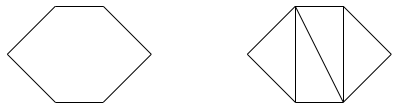
\includegraphics[width=0.6\textwidth]{./Introduction/hex_tri_cells}
\caption{Hexagonal cell versus triangle cells}
\label{fig_hex_tri}
\end{figure}
We see in Figure \ref{fig_hex_tri} that if there is one unknown per vertex, 
the hexagonal cell will have 6
unknowns compared to the 12 unknowns of triangle cells. Polygonal cells can
also be used for adaptive mesh refinement (AMR) without having to
deal with hanging nodes 
\cite{locally_hanging_nodes,arbitrary_hanging_nodes,dealII_hanging_nodes}. The 
left cell on the Figure \ref{fig_amr_mesh} is a degenerate pentagon whereas 
the two cells on the right are quadrilaterals:
\begin{figure}[H]
\centering

\includegraphics[width=0.4\textwidth]{./Introduction/amr}
\caption{AMR mesh}
\label{fig_amr_mesh}
\end{figure}

\section{Linear Boltzmann equation}
Charged particles transport can be described by the linear Boltzmann equation 
\cite{cepxs,galerkin_morel,morel_81}:
\begin{equation}
  \begin{split}
    \bo\cdot \bn \psi(\br,\bo,E) + \Sigma_t(\br,E)\psi(\br,\bo,E) = 
    \int_0^{\infty}dE'\int_{4\pi}d\bo'&  \\
     \Sigma_s(\br,\bo'\cdot\bo,E'\rightarrow E)
     \psi(\br,\bo',E')&+Q(\br,\bo,E)
  \end{split}
\label{transport_p}
\end{equation}
where:
\begin{itemize}
\item $\bo = (\mu,\varphi)$ is a unit vector in the flight direction
\item $\mu = \cos(\theta)$, where $\theta$ is the directional polar angle
\item $\varphi$ is the directional azimuthal angle
\item $\mu_0 = \bo'\cdot \bo$ 
\item $\psi(\br,\bo,E) = vf(\br,\bo,E)$ is the angular flux
\item $\Sigma_t(\br,E)$ is the total macroscopic cross section given by:
\begin{equation}
\Sigma_t(\br,E) = \Sigma_a(\br,E)+\Sigma_s(\br,E)
\end{equation}
\item $\Sigma_a(\br,E)$ is the absorption macroscopic cross section
\item $\Sigma_s(\br,E)$ is the scattering macroscopic cross section
\item $\Sigma_s(\br,\bo'\cdot \bo, E'\rightarrow E)$ is the differential
scattering macroscopic cross scattering
\item $Q(\br,\bo,E)$ is the volumetric source
\end{itemize}
In the rest of this work, macroscopic cross sections will simply be called cross
sections when no confusion is possible. Standard boundary conditions can be
applied to \cref{transport_p}. The most common is the incoming flux boundary
condition:
\begin{equation}
  \psi (\br,\bo,E) = g(\br,\bo,E) \textrm{ for }\bo \cdot \bs{n} <0 \textrm{ and }
\br \in \partial \mc{D},
\label{bc}
\end{equation}
where $\partial \mc{D}$ is the boundary of the domain $\mc{D}$. If $g=0$, 
\cref{bc} yields the vacuum boundary conditions.

\Cref{transport_p} depends on space $(\br)$, angle ($\bo$), and 
energy $(E)$. In practice, the energy variable is treated through a
multigroup formalism, with outer iterations between all energy groups to
include down/up scattering events (including transfers between particle
types). The multigroup equations are solved one at a time, yielding a
within-group transport problem. This within-group problem retains the 
challenging features of the electron-photon problem we want to address. 
As such, the methods developed here will be presented for the within-group 
transport equation. However, the techniques described here apply 
straightforwardly to the multigroup equations. The energy-integrated 
\cref{transport_p} is given by:
\begin{equation}
\bo\cdot \bn \psi(\br,\bo) + \Sigma_t(\br)\psi(\br,\bo) =
\int_{4\pi}d\bo'\ \Sigma_s(\br,\bo'\cdot\bo)\psi(\br,\bo')+Q(\br,\bo).
\label{transport_p2}
\end{equation}
%
Using:
\begin{align}
  &\Sigma_s(\br,\bo\cdot\bo') = \sum_{l=0}^{\infty} \frac{2l+1}{4\pi}
  \Sigma_{s,l}(\br) P_l(\bo\cdot\bo')\\
  &\Sigma_{s,l}(\br) = 2\pi \int_{-1}^1 d\mu_0\ P_l(\mu_0)
  \Sigma_s(\br,\mu_0),
\end{align}
the scattering term can be represented by a Legendre polynomials $P_l$ expansion:
\begin{equation}
  \int_{4\pi} \Sigma_s(\br,\bo'\cdot\bo) \psi(\br,\bo') d\bo' =
  \int_{4\pi} \sum_{l=0}^{\infty} \frac{2l+1}{4\pi} \Sigma_{s,l} P_l(\bo'\cdot\bo)
  \psi(\br,\bo') d\bo'.
  \label{scatt_d_1}
\end{equation}
Using the addition theorem for spherical harmonics, $Y_l^m$ the spherical
harmonics of degree $l$ and order $m$, and $P_l^m$ the associated Legendre
polynomials:
\begin{align}
  & P_l(\bo\cdot\bo') = \frac{4\pi}{2l+1} \sum_{m=-l}^l
  Y_l^m(\bo)Y_l^{m,*}(\bo')\\
  & Y_l^m(\bo) = (-1)^m \sqrt{\frac{2l+1}{4\pi} \frac{(l-m)!}{(l+m)!}} P_l^m(\mu)
  e^{im\varphi},
\end{align}
\cref{scatt_d_1} becomes:
\begin{equation}
  \begin{split}
    \int_{4\pi} \Sigma_s(\br,\bo'\cdot\bo) \psi(\br,\bo') d\bo' &=
    \int_{4\pi} \sum_{l=0}^{\infty} \frac{2l+1}{4\pi}\frac{4\pi}{2l+1}
    \Sigma_{s,l}(\br) \\
    &\quad \sum_{m=-l}^{l} Y_l^m(\bo)Y_l^{m,*}(\bo') \psi(\br,\bo')d\bo'\\
    &= \sum_{l=0}^{\infty} \Sigma_{s,l}(\br) \sum_{m=l}^l \phi_{l,m}(\br)
    Y_l^m(\bo),
  \end{split}
\end{equation}
where we have introduced:
\begin{align}
&\psi(\br,\bo) = \sum_{l=0}^{\infty}\sum_{m=-l}^l \phi_{l,m}(\br) Y_l^m(\bo),
\label{ang_flux}\\
&\phi_{l,m}(\br) = \int_{4\pi} d\bo\ Y_{l}^{m,*}(\bo) \psi(\br,\bo).
\label{moments}
\end{align}
In practice, the scattering expansion is 
truncated $(\sum_{l=0}^{\infty}\rightarrow \sum_{l=0}^L)$.\\
For the derivation of the Boltzmann-Fokker-Planck equation, we will need the 
following property of the spherical harmonics:
\begin{equation}
\[\frac{\partial}{\partial\mu}(1-\mu^2)\frac{\partial}{\partial
\mu}+\(\frac{1}{1-\mu^2}\)\frac{\partial^2}{\partial
\varphi}+l(l+1)\]Y_l^m(\bo)=0.
\label{eigenvalue}
\end{equation}
\Cref{transport_p2} still needs to be discretized in space and angle. A
standard method to discretize the space variable is to use discontinuous
Galerkin finite elements \cite{thick_dgfem,conv_dgfem,dgfem}. The angular
discretization that we will use in this work is the $S_n$ or discrete ordinate
method \cite{sn_sandia,sn_var,sn_equiv,rad_transfer}. With this 
discretization, \cref{transport_p2} is replaced by a system of linear equations 
which use discrete angular fluxes $\(\psi(\br,\bo)\rightarrow 
\psi(\br,\bo_d)=\psi_d(\br)\)$ and the integral in \cref{moments} is replaced 
by a quadrature:
\begin{equation}
\phi_{l,m}(\br) = \sum_d w_d Y_{l}^{m,*}(\bo_d) \psi_d(\br),
\label{moments_2}
\end{equation}
where $w_d$ are the weights associated to the quadrature. Therefore, the $S_n$
discretization of \cref{transport_p2} is given by:
\begin{equation}
\bo_d\cdot\bn \psi_d(\br) + \Sigma_t(\br)\psi_d(\br) = \sum_{l=0}^L
\Sigma_{s,l}(\br) \sum_{m=-l}^l \phi_{l,m} Y_l^m(\bo_d) + Q_d(\br).
\label{transport_sn}
\end{equation}
\Cref{transport_sn} can be written in a more compact way using operators:
\begin{equation}
  \bs{L}\Psi = \bs{M}\bs{\Sigma}\bs{D}\Psi + Q
\label{transport_operator}
\end{equation}
where:
\begin{itemize}
  \item $\bs{L}$ is the streaming operator $\bo_d \cdot \bn + \Sigma_t(\br)$
  \item $\bs{M}$ is the moment-to-direction operator $\Psi = \bs{M}\Phi$
  \item $\bs{D}$ is the direction-to-moment operator $\Phi = \bs{D}\Psi$
  \item $\bs{\Sigma}$ is the scattering cross-section operator
  \item $\Psi$ is the vector of angular fluxes $\psi_d$
  \item $\Phi$ is the vector of angular flux moments $\phi_{l,m}$.
\end{itemize}


\section{Organization of the Dissertation}
\noindent In Chapter \ref{cp_transport_chapter}, we introduce the 
Boltzmann-Fokker-Planck (BFP) equation used to describe the transport of
charged particles. To obtain the BFP equation, the Fokker-Planck operator is
added in the Boltzmann equation in order to simplify the treatment of the
highly forward-peaked scattering kernel. We show that the Fokker-Planck
equation is an asymptotic limit of the Boltzmann equation when the mean free
path goes to zero and $\bar{\mu}_0$ goes to one. The Fokker-Planck equation is
not valid for any forward-peaked scattering kernel and therefore, the BFP
approximation has some limitations. In particular, the Henyey-Greenstein
kernel and the Rutherford cross section do not satisfy the Fokker-Planck
limit. Being aware of these limitations, we introduce the Fokker-Planck cross
section that allows to reduce the Fokker-Planck equation and the BFP equation
to a Boltzmann equation. Fokker-Planck cross sections cannot be used with any
angular $S_n$ quadrature but specific quadratures, known as Galerkin
quadratures, must be adopted. The importance and the properties of these
quadratures are explained in details at the end of Chapter
\ref{cp_transport_chapter}.

In Chapter \ref{spatial_chapter}, we review in details the iterative
solvers and the spatial discretizations used to solve the $S_n$ transport 
equations. We explain how Source Iteration, Krylov solvers, and Diffusion 
Synthetic Acceleration can be used to solve the transport equation.
We introduce two spatial discretizations for 2D geometries: BiLinear 
Discontinuous finite elements (BLD) and PieceWise 
Linear Discontinuous finite elements (PWLD). The BLD finite elements are used 
on rectangular cells while the PWLD finite elements can be used on any polygonal 
cells. The purpose of this Chapter is to facilitate expansion in the next
Chapter.

In Chapter \ref{anmg_chapter}, we introduce the angular multigrid 
methods for transport with highly forward-peaked scattering. We recall  
prior work on this topic and discuss the issues previously encountered for 
multidimensional geometries. The original angular multigrid method for 
one-dimensional geometry showed rapid convergence of source iterations for 
problems with highly forward-peaked scattering, whereas the standard SI+DSA
approach is ineffective. Unfortunately, the 
generalization to multidimensional geometries required a filter to stabilized 
the method which resulted in a significantly less efficient scheme than in 
one-dimensional geometry. When 
the scattering becomes very anisotropic, this generalized method becomes
ineffective. In this Chapter, we show that if the angular multigrid method is 
recast as a preconditioner for a Krylov solver, the method does not need 
diffusion filtering for stability and is always effective and efficient.

In Chapter \ref{mip_chapter}, we adapt the Modified Interior 
Penalty (MIP) DSA developed for triangular cells to quadrilateral and polygonal 
cells. This DSA discretization is used as the coarsest level of the angular 
multigrid method developed in Chapter \ref{anmg_chapter}. Since MIP is
symmetric and positive-definite, the most common method to solve it, is to use
conjugate gradient (CG) preconditioned by SSOR. In Chapter \ref{mip_chapter}, we 
investigate algebraic multigrid methods as CG preconditioners to solve MIP. 
We show that algebraic multigrid preconditioners are vastly superior to more
common CG preconditioners if the matrix associated to MIP is stored.

In Chapter \ref{janus_chapter}, the implementation of the code
developed for this research is detailed.

In Chapter \ref{conclusion_chapter}, we finish with some concluding 
remarks and suggestions for future developments.
